\documentclass[tikz,border=6pt]{standalone}
\usepackage{amsmath,amssymb}
\usepackage{tikz}
\usetikzlibrary{arrows.meta,calc,decorations.pathreplacing,patterns,shapes.geometric,positioning,shadings}

\begin{document}
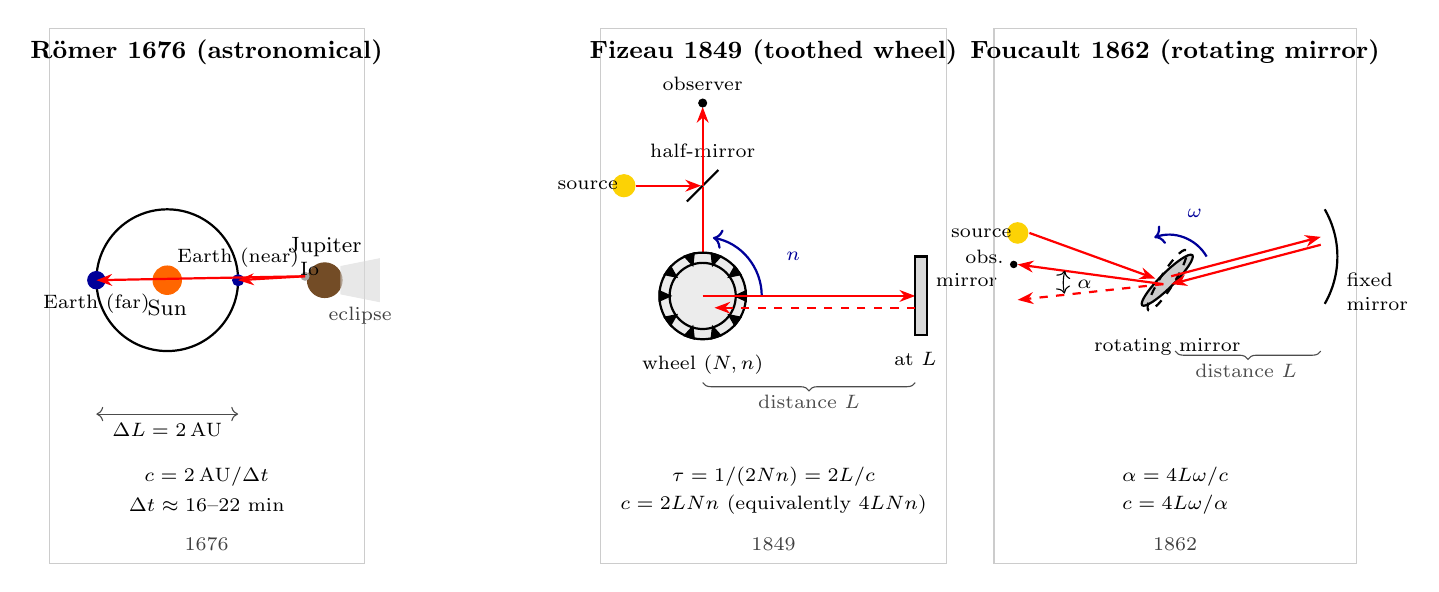
\begin{tikzpicture}[
  font=\footnotesize,
  every node/.style={inner sep=1pt},
  ray/.style={red, thick, -{Stealth[length=2mm]}},
  raydash/.style={red, thick, dashed, -{Stealth[length=2mm]}},
  instrument/.style={black, thick},
  thinline/.style={black, thin},
]

% ============================================================
% LEFT PANEL: Roemer 1676
% ============================================================
\begin{scope}[shift={(0,0)}]
  % Panel frame
  \draw[thinline, gray!40] (-4.2,-3.6) rectangle (-0.2,3.2);
  \node[black, font=\small\bfseries] at (-2.2, 2.9) {R\"omer 1676 (astronomical)};

  % Sun
  \filldraw[orange!80!red] (-2.7,0) circle (0.18);
  \node[below=2pt] at (-2.7,-0.15) {Sun};

  % Earth orbit
  \draw[instrument] (-2.7,0) circle (0.9);

  % Earth near (closest to Jupiter side) -- to the right (toward Jupiter)
  \filldraw[blue!60!black] (-1.8,0) circle (0.07);
  \node[above=1pt, font=\scriptsize] at (-1.8,0.08) {Earth (near)};

  % Earth far -- opposite side
  \filldraw[blue!60!black] (-3.6,0) circle (0.11);
  \node[below=1pt, font=\scriptsize] at (-3.6,-0.1) {Earth (far)};

  % Jupiter (outside, to the right)
  \filldraw[brown!60!black] (-0.7,0) circle (0.22);
  \node[above=1pt] at (-0.7,0.22) {Jupiter};

  % Io (small moon) and shadow
  \filldraw[gray!70] (-0.95,0.05) circle (0.05);
  \node[font=\scriptsize, above right=-1pt and -3pt] at (-0.95,0.05) {Io};
  % Shadow cone behind Jupiter (to the right, opposite Sun)
  \fill[gray!30, opacity=0.6] (-0.5,-0.18) -- (0.0,-0.28) -- (0.0,0.28) -- (-0.5,0.18) -- cycle;
  \node[font=\scriptsize, gray!50!black] at (-0.25,-0.45) {eclipse};

  % Light rays from Io to two Earth positions
  \draw[ray] (-0.95,0.05) -- (-1.8,0.0);
  \draw[ray] (-0.95,0.05) -- (-3.6,0.0);

  % Labels
  \draw[<->, thin, gray!60!black] (-3.6,-1.7) -- (-1.8,-1.7);
  \node[font=\scriptsize] at (-2.7,-1.9) {$\Delta L = 2\,\mathrm{AU}$};

  \node[font=\scriptsize] at (-2.2,-2.5) {$c = 2\,\mathrm{AU}/\Delta t$};
  \node[font=\scriptsize] at (-2.2,-2.85) {$\Delta t \approx 16\text{--}22$ min};

  \node[gray!50!black, font=\scriptsize] at (-2.2,-3.35) {1676};
\end{scope}

% ============================================================
% MIDDLE PANEL: Fizeau 1849 gear wheel
% ============================================================
\begin{scope}[shift={(5,0)}]
  \draw[thinline, gray!40] (-2.2,-3.6) rectangle (2.2,3.2);
  \node[black, font=\small\bfseries] at (0, 2.9) {Fizeau 1849 (toothed wheel)};

  % Light source (left)
  \filldraw[yellow!70!orange] (-1.9,1.2) circle (0.14);
  \node[font=\scriptsize, left=1pt] at (-1.9,1.2) {source};

  % Half-silvered mirror (45 deg) at (-0.9, 1.2)
  \draw[instrument, thick] (-1.1,1.0) -- (-0.7,1.4);
  \node[font=\scriptsize, above=2pt] at (-0.9,1.45) {half-mirror};

  % Ray from source to half-mirror then bending down to wheel
  \draw[ray] (-1.75,1.2) -- (-0.92,1.2);
  \draw[ray] (-0.9,1.18) -- (-0.9,0.05);

  % Toothed wheel at (-0.9, -0.2), side view (vertical gear)
  \def\wheelR{0.55}
  \def\wheelr{0.42}
  \def\Nt{10}
  \draw[instrument, fill=gray!15] (-0.9,-0.2) circle (\wheelR);
  \draw[instrument] (-0.9,-0.2) circle (\wheelr);
  % teeth as radial marks
  \foreach \k in {0,1,...,9}{
    \pgfmathsetmacro{\ang}{36*\k}
    \draw[instrument, fill=black] ({-0.9+\wheelr*cos(\ang)},{-0.2+\wheelr*sin(\ang)})
      -- ({-0.9+\wheelR*cos(\ang+6)},{-0.2+\wheelR*sin(\ang+6)})
      -- ({-0.9+\wheelR*cos(\ang-6)},{-0.2+\wheelR*sin(\ang-6)}) -- cycle;
  }
  % Rotation arrow
  \draw[->, thick, blue!60!black] (-0.15,-0.2) arc[start angle=0, end angle=80, radius=0.75];
  \node[blue!60!black, font=\scriptsize] at (0.25,0.3) {$n$};

  % label
  \node[font=\scriptsize, below=3pt] at (-0.9,-0.8) {wheel $(N,n)$};

  % Beam continues to the right through gap
  \draw[ray] (-0.9,-0.2) -- (1.8,-0.2);
  % Distant mirror
  \draw[instrument, thick] (1.8,-0.7) -- (1.8,0.3);
  \draw[instrument, thick, fill=gray!30] (1.8,-0.7) rectangle (1.95,0.3);
  \node[font=\scriptsize, right=2pt] at (1.95,0.0) {mirror};
  \node[font=\scriptsize] at (1.8,-1.0) {at $L$};

  % Distance bracket
  \draw[decorate, decoration={brace, amplitude=3pt, mirror}, gray!60!black]
    (-0.9,-1.3) -- (1.8,-1.3);
  \node[font=\scriptsize, gray!60!black] at (0.45,-1.55) {distance $L$};

  % Return beam (slightly offset) blocked by next tooth: dashed segment at wheel
  \draw[raydash] (1.8,-0.35) -- (-0.75,-0.35);

  % Observer below half-mirror
  \draw[ray] (-0.9,1.2) -- (-0.9,2.2);
  \filldraw[black] (-0.9,2.25) circle (0.05);
  \node[font=\scriptsize, above=2pt] at (-0.9,2.3) {observer};

  % Formula
  \node[font=\scriptsize] at (0,-2.5) {$\tau = 1/(2Nn) = 2L/c$};
  \node[font=\scriptsize] at (0,-2.85) {$c = 2LN n$ (equivalently $4LN n$)};

  \node[gray!50!black, font=\scriptsize] at (0,-3.35) {1849};
\end{scope}

% ============================================================
% RIGHT PANEL: Foucault 1862 rotating mirror
% ============================================================
\begin{scope}[shift={(10,0)}]
  \draw[thinline, gray!40] (-2.2,-3.6) rectangle (2.4,3.2);
  \node[black, font=\small\bfseries] at (0.1, 2.9) {Foucault 1862 (rotating mirror)};

  % Light source (left)
  \filldraw[yellow!70!orange] (-1.9,0.6) circle (0.13);
  \node[font=\scriptsize, left=1pt] at (-1.9,0.6) {source};

  % Ray from source to rotating mirror
  \draw[ray] (-1.75,0.6) -- (-0.15,0.02);

  % Rotating mirror at origin (small ellipse, 45 deg)
  \draw[instrument, fill=gray!40, rotate around={45:(0,0)}] (0,0) ellipse (0.45 and 0.09);
  % Virtual later position (dashed)
  \draw[instrument, dashed, rotate around={58:(0,0)}] (0,0) ellipse (0.45 and 0.09);
  % rotation arrow and omega
  \draw[->, thick, blue!60!black] (0.5,0.3) arc[start angle=30, end angle=110, radius=0.55];
  \node[blue!60!black, font=\scriptsize] at (0.35,0.85) {$\omega$};
  \node[font=\scriptsize, below=14pt] at (0,-0.2) {rotating mirror};

  % Ray to distant curved mirror on the right
  \draw[ray] (0.05,0.05) -- (1.95,0.55);

  % Fixed concave mirror at right
  \draw[instrument, thick] (2.0,-0.3) arc[start angle=-30, end angle=30, radius=1.2];
  \node[font=\scriptsize, right=1pt] at (2.2,0.0) {fixed};
  \node[font=\scriptsize, right=1pt] at (2.2,-0.3) {mirror};

  % Distance label
  \draw[decorate, decoration={brace, amplitude=3pt, mirror}, gray!60!black]
    (0.1,-0.9) -- (1.95,-0.9);
  \node[font=\scriptsize, gray!60!black] at (1.0,-1.15) {distance $L$};

  % Return ray along same path then deflected by alpha on way back
  \draw[ray] (1.95,0.45) -- (0.05,-0.05); % back to rotating mirror
  % reflected back toward observer but deflected by 2*theta = alpha
  \draw[ray] (-0.05,-0.05) -- (-1.9,0.2); % original return direction (going to observer)
  \draw[raydash] (-0.05,-0.05) -- (-1.9,-0.25); % deflected direction (alpha)

  % alpha angle arc
  \draw[<->, thin, black] (-1.3,0.12) arc[start angle=165, end angle=193, radius=0.6];
  \node[font=\scriptsize] at (-1.05,-0.05) {$\alpha$};

  % observer
  \filldraw[black] (-1.95,0.2) circle (0.04);
  \node[font=\scriptsize, left=1pt] at (-2.0,0.3) {obs.};

  % Formula
  \node[font=\scriptsize] at (0.1,-2.5) {$\alpha = 4L\omega/c$};
  \node[font=\scriptsize] at (0.1,-2.85) {$c = 4L\omega/\alpha$};

  \node[gray!50!black, font=\scriptsize] at (0.1,-3.35) {1862};
\end{scope}

\end{tikzpicture}
\end{document}
